\section{\I{The population section}\label{sec:population-section}}

\subsection{Introduction}
The population section\index{Population section} specifies the model structure, population dynamics, and other associated parameters. It describes the model structure (population structure), defines the population processes (e.g., recruitment, migration, and mortality), selectivities, and model parameters.

The population section consists of several components, including;
\begin{itemize}
  \item The population structure;
  \item Model initialisation (i.e., the state of the model at the start of the first year)\index{Initialisation}\index{Model ! initialisation};
  \item The years over which the model runs (i.e., the start and end years of the model)
  \item The annual cycle (time-steps and processes that are applied in each time-step)\index{Annual cycle};
  \item The specifications and parameters of the population processes (i.e. processes that add, remove individuals to or from the partition, or shift numbers between ages and categories in the partition);
  \item Selectivities;
  \item Parameter values and their definitions;
  \item Derived quantities, required as parameters for some processes (e.g. spawning stock biomass to resolve the spawner-recruit relationship in a recruitment process).
\end{itemize}


\subsection{\I{Population structure}}

The basic structure of a \CNAME\ population model is defined in terms of an annual cycle, time steps, states, and transitions.

The annual cycle defines what processes happen in each model year, and in what sequence. (In line with the New Zealand fisheries management framework, \CNAME\ runs on an annual cycle rather than, for example, a 6-monthly cycle.) 

Each year is split into one or more time steps, with at least one process occurring in each time step. Each time step can be thought of as representing a particular part of the calendar year, or you can just treat them as an abstract sequence of events.\hlc[new]{In every time step, there exists a mortality block, this is a block where individuals are removed from the partition. If there are no mortality processes then the mortality block is empty (nothing happens) and occurs at the end of a time step}. maybe the user doesn't need to know this more of a code base statement

The state is the current status of the population, at any given time. The state can change one or more times in every time step of every year. The state object must contain sufficient information to figure out the future course of the fishery (given a model and a complete set of parameters).

There are a number of possible changes in the state, which are called transitions. These include processes such as recruitment, natural mortality, fishing mortality, ageing, migration, tagging events, and maturation.

The division of the year into an arbitrary number of time steps allows the user to specify the exact order in which processes and observations occur. The user needs to specify the time step in which each process occurs. If more than one process occurs in the same time step, they will be applied in the order specified in the \command{time\_step} block.

The key element of the state is the partition. This is a broadly applicable concept that can be used to describe many different kinds of population model. The partition is simply a breakdown of the total number of fish in the current population into different kinds of fish (Note that the partition records numbers of fish, not biomass). The fish are categorised by various characters. Traditionally these characters have been: length class or age class, sex, maturity, area, stock, tag, and growth-path. However \CNAME\ has no predefined characters in the partition. This is a major extension on CASAL where users can extend on traditional problems, for example incorporating predator, prey, and in the case of some shellfish species a clock(dead) category. 


When defining the partition the user must choose:
\begin{itemize}
\item	whether the partition is subdivided by length class or age class (not both)
\item	which of the other characters are included in the partition, e.g., the number of areas, stocks, tagging events, or growth paths (if any of these characters are included in the partition).
\end{itemize}
\hlc{
The resulting partition can be conceptualised as a matrix, where the columns are length or age classes and the rows represent combinations of the other characters. Then the number in each cell of the matrix is the number of fish with the corresponding combination of characters.}\\ 
\textbf{Craigs attempt}\\
\hlc[new]{The resulting partition can be conceptualised as a group of vectors, where each category is represented as a vector and the size of the vector is the number of age or length classes, shown in Figure~4.1. Each element in a vector represents the number of individuals for that category in that age or length bin. splitting the partition up into separate categories allows categories to have different age or length structures.
	
The names and number of categories are user defined, but there must be at least one category defined for a model. The ages are defined as a sequence from $age_{min}$ to $age_{max}$, with the last age optionally a plus group. In order to calculate biomass, the age-length relationship for each category must also be defined. An example of how this is specified for four categories based on sex and area is as follows,}
{\small{\begin{verbatim}
	@categories 
	format mature.sex
	names 		spawn.male 	spawn.female 	nonspawn.male 	nonspawn.female
	age_lengths 	male_AL		female_AL   male_AL		female_AL  
		\end{verbatim}}}	

For an example of these ideas, consider a model of a single stock with a spawning and non-spawning fishery. The non-spawning fishery happens over most of the year (say 10 months) in the home area. The mature fish then migrate to the spawning area, where the spawning fishery operates. At the end of spawning, these fish, along with the recruits from the previous year, migrate back to the home area. The modeller decides that fish will be divided in the partition by age, sex, maturity, and area (spawning and home grounds). So the partition has 8 rows (2 sexes × (mature or immature) × 2 areas) and one column per age class. 

For an example of these ideas, consider a model of a single stock with a spawning and non-spawning fishery. The non-spawning fishery happens over most of the year (say 10 months) in the home area. The mature fish then migrate to the spawning area, where the spawning fishery operates. At the end of spawning, these fish, along with the recruits from the previous year, migrate back to the home area. The modeller decides that fish will be divided in the partition by age, sex, maturity, and area (spawning and home grounds). So the partition has 8 rows (2 sexes × (mature or immature) × 2 areas) and one column per age class. 
\begin{figure}[H]\label{Fig:part}
	\centering
	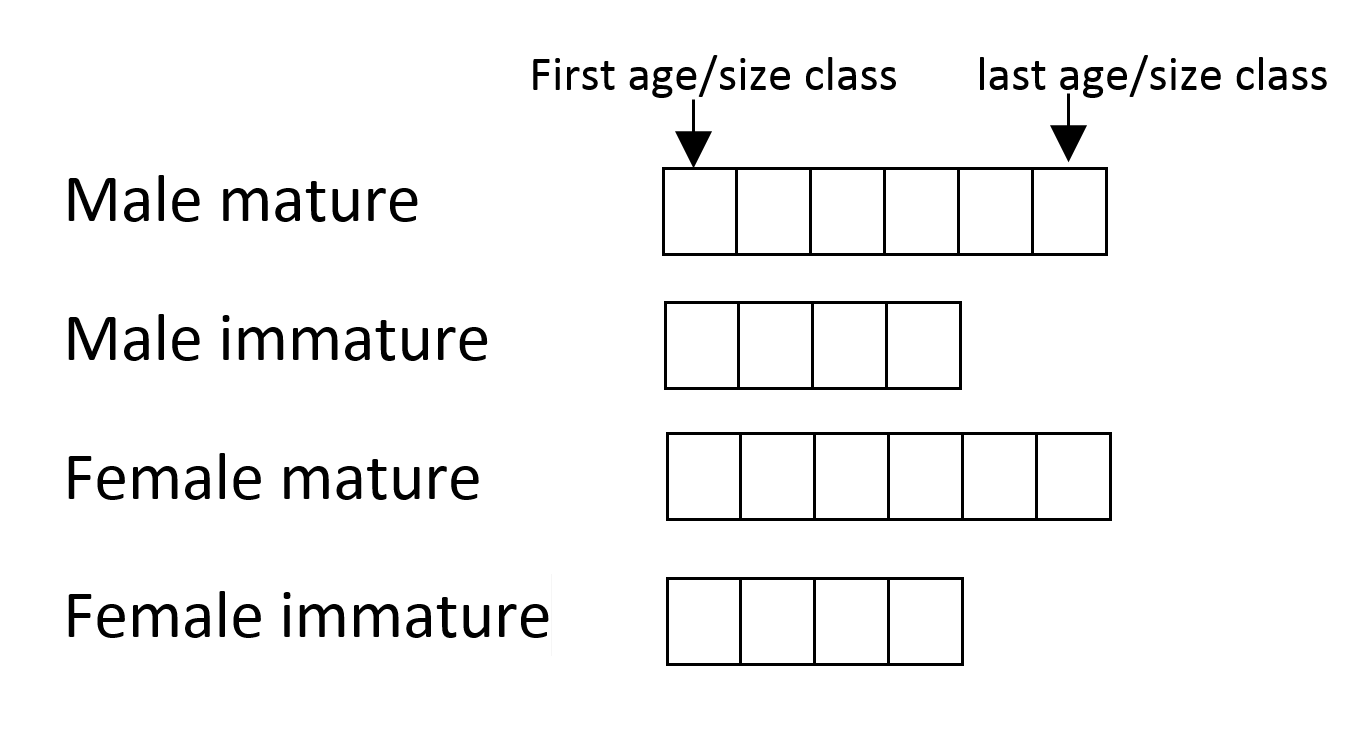
\includegraphics[scale=0.3]{Figures/partition.png}
		\caption{A visual representation of a partition}
\end{figure}


So they define four time steps, labelled 1 through 4. Step 1 includes the non-spawning fishery. Step 2 includes the migration to the spawning area. Step 3 includes the spawning fishery. Step 4 includes recruitment and the migration back to the home area. (In fact, they could have used only 3 time steps, by using a single step in place of their steps 2 and 3. Because the default order of processes within a time step places migrations before fisheries, the processes would still have occurred in the right order.) There are other details to be sorted out, such as the proportion of natural mortality occurring in each time step, but this gives the basic idea. 

This structure can be used to implement complex models, with intermingling of separate stocks, with complex migration patterns over multiple areas, and multiple fisheries using different fishing methods and covering different areas and times. Note that there is little point in using a complex structure to model a stock when there are no observations to support that structure. In other words, use a structure for your model that is compatible with the data available. 

The model is run from an initial year up to the final(current) year. It can also be run past the final year to make projections — things that happen in the future — up to the final projection year.

An example, to specify a model with 2 categories (male and female) with ages 1-20 (with the last age a plus group) and an age-length relationship defined with the label \texttt{male\_growth} and \texttt{female\_growth}, then the \texttt{@model} example from above becomes,
{\small{\begin{verbatim}
		@model
		start_year
		final_year
		min_age 1
		max_age 20
		age_plus_group True
		initialisation_phases iphase
		time_steps step1 step2
		\end{verbatim}}}

\subsection{\I{The state object and the partition}}

\hl{The key component of the state object is the partition, a matrix of numbers of fish by combinations of characters. The columns can either be age or length classes, the rows are combinations of the following characters:}

\hlc[new]{The key component of the state object is the partition, a group of vectors that store numbers of fish at age or length for a specific category. A category represents a group of fish that have specific attributes, examples of such attributes include life histories and growth paths. Characters in a population that display different attributes and that can make up a category or seperate categories are:}

\begin{itemize}
\item Sex (male or female);
\item Area (any number of areas, named by the user);
\item Stock (any number of stocks, named by the user);
\item Maturity (immature or mature);
\item Growth-path (any number of growth-paths);
\item Tag. (any number of tagging events).
\end{itemize}

A stock is defined as a subpopulation of fish which recruits separately. See Section \ref{sec:maturity-notinpartition} for the treatment of maturity when it is not a character in the partition. 

Growth-paths are a feature used to implement some persistence of length at age in an age-based model that uses some length/size data. Each growth-path has its own growth curve, and the length-based model features will consequently  have different effects on different growth-paths. So, you need to tell \CNAME\ the following: 

\begin{itemize}
\item Whether the model is age- or length-based.
\item The number and nature of length classes in a length-based model.
\item	The minimum and maximum age classes in an age-based model.
\item	Whether there is a plus group.
\item 	The names of all categories and there corresponding growth path labels.
\item	Whether the partition is divided by sex.
\item	Whether the partition is divided by maturity.
\item	Whether the partition has growth-paths, and, if so, how many.
\item	Whether the partition has multiple stocks, and, if so, how many, and their names.
\item	Whether the partition has multiple areas, and, if so, how many, and their names.
\item	Whether the partition includes tagged fish, and, if so, how many, and the names of the tag partitions.
\end{itemize}

Age classes are always 1 year wide, except that the maximum age group can optionally be a plus group. Users need to choose the minimum and maximum age classes. Length classes are defined by the user, and you need to specify how many length classes there are, the lower bound of each length class, and whether the last length class is a plus group, or if not, what its upper bound is. The relevant parameters are \texttt{class\_mins} and \texttt{plus\_group}. The \texttt{class\_mins} parameter contains the lower bound of each class, and concludes with the upper bound of the last class if it is not a plus group. If, for example, length classes of 30-40, 40-50, 50-60, and 60-70+ cm were desired, you would set \texttt{class\_mins 30 40 50 60} and \texttt{plus\_group true}. Whereas if 30-40, 40-50, 50-60, and 60-70 cm were desired, you would set \texttt{class\_mins 30 40 50 60 70} and \texttt{plus\_group false}.

\CNAME\ allows categories of the partition to exist for certain years of the model. This is added for computational efficiency, when models contain a large number of categories that do not persist for all model years. Situations where this is beneficial is when a model contains a process that transitions fish into a category that has otherwise not been used, for example tagging events. Excluding categories for certain years saves initialising empty categories. This can be a big time saver if initialisation is run for 50 years and there are many tagging events.(When the ross sea model is up and running \% differences would be a nice insert here)

Another important component of the state object in \texttt{casal$^2$} are derived quantities. This includes quantities such as spawning stock biomasses (SSBs, mid-spawning season biomasses of spawning fish) for each or a combination of categories. \texttt{Casal$^2$} derives through the command \command{derived\_quantity}, this is needed if there is a stock-recruitment relationship.

\subsection{\I{Time sequences}}

The time sequence of the model is defined in three parts;
\begin{itemize}
  \item \I{Initialisation}
  \item \I{Run years}
  \item \I{Projection year}s
\end{itemize}

\subsubsection{\I{Annual cycle}}

The annual cycle is implemented as a set of processes that occur, in a user-defined order, within each year. Time-steps are used to break the annual cycle into separate components, and allow observations to be associated with different sets of processes. Any number of processes can occur within each time-step, in any order and can occur multiple times within each time-step. Note that time-steps are not implemented during the initialisation phases (effectively, there is only one time-step), and that the annual cycle in the initialisation phases can be different from that which is applied during the model years.

\subsubsection{\I{Initialisation}}

There are multiple methods to initialise a partition in \CNAME. These methods are: iterative, fixed, derived and Cinitial. Model initialisation can occur in several phases\index{Initialisation!phases}, each of which can be a different type. At the end of the initialisation step, \CNAME\ runs through the model years carrying out processes in the order defined in the annual cycle, and can evaluate expected values of observations in order to calculate likelihoods, project forward to determine future states, or simulate observations from the current state.

\subsubsection*{\I{Iterative Intitialisation}}
One of \CNAME\ methods for initialising the initial equilibrium state as an iterative process: a general solution that initialises complex structured models can be difficult to implement using analytic techniques. However, initialising via iteration for a long-lived species with complex transitions can take many iterations and be slow to run. In \CNAME, we allow for user-defined multi-phased initialisation using iteration to allow the user to optimize models for speed. Each phase of the initialisation can involve any number of processes. Note that the length of the initialisation period may affect the model outputs, and that a period should be chosen to allow the population state to converge.

In addition, each initialisation process can optionally be stopped early if a user defined convergence criteria is met. For a set of user defined years in the initialisation phase, convergence is defined as met if the proportional absolute summed difference between the the state in year $t-1$ and the state in year $t$ ($\widehat{\lambda}$) is less than $\lambda$ where, 
\begin{equation}
  \widehat{\lambda} = \frac{\sum\limits_{i} \sum\limits_{j} \left|\text{element}(i,j)_t - \text{element}(i,j)_{t-1} \right|}{\sum\limits_{i} \sum\limits_{j} \frac{}{}\text{element}(i,j)_t}
\end{equation}

In each initialisation phase, the processes defined for that phase are carried out and used as the starting point for the following phase or, if it is the last phase, then the years that the model is run over. The first phase is always initialised with each element (i.e., each age and category) set at zero. Note that this means that recruitment processes where the numbers of recruits is based on a stock recruitment or density dependant relationship will likely fail if used in the first phase of an initialisation. 

The multi-phase iteration\index{Multi-phase iteration} allows the user to determine if the initialisation has converged in a particular model run. Here, add an additional initialisation phase for, say, $1$ year as the last initialisation phase (with the same processes applied). Then, using the initialisation reports (\commandlabsubarg{report}{type}{initialisation\_partition}), print a copy of the partition just before and just after that phase. If the initialisation has converged to an equilibrium state, then the partition at both these time intervals will be the same.

Hence, for an iterative initialisation you need to define;
\begin{itemize}
  \item The initialisation phases.
  \item The number of years in each phase and the processes to apply in each (default is the annual cycle).
\end{itemize}
\subsubsection*{\I{Derived Intitialisation}}
An analytical solution to the iterative initialisation phase. It can be solved in max\_age - min\_age +1 years. 
\subsubsection*{\I{Cinitial Intitialisation}}
This phase can only be applied once a derived or iterative intialisation phases has been implemented. It works off an equilibrium state and usese Cinitial factors that can be estimated to shift the intial population away from equilibrium prior to start year. This is implemented in teh Southern Blue Whiting assessment a FAR reference would be nice (AListair)
\subsubsection*{\I{Fixed Intitialisation}}
This is a user defined table that is taken to be the initial partition prior to start year.
\subsubsection*{\I{Model years}}

Following initialisation, the model then runs over a number of user-defined years. For this part of the model, the annual cycle can be broken into separate time-steps, and observations can be associated with the state of the model at the end of any time-step, i.e., likelihoods for particular observations are evaluated, if required, at the end of each time-step. 

Processes are carried out in the order specified within each time-step, and can be the same or different to processes in other initialisation phases of the model. The run years define the years over which the model is to run and the annual cycle within each year. The model runs from the start of year \argument{initial} and runs to the end of year \argument{current}. The projection part then extends the run time up to the end of year \argument{final}. 

\begin{itemize}
  \item The time-steps and the processes applied in each
  \item The initial year (i.e., the model start year)
  \item The final year (i.e., the model end year)
  \item The projection final year (i.e., the model projection end year)
\end{itemize}

\subsubsection{\I{Projections}\label{sec:projections}}

\CNAME\ can project, from a set of parameter estimates, the state of the model into the future. In a projection run, the model is initialised and run through the model years from \argument{initial} to the \argument{final}. Then, the model is re run from \argument{intial} to \argument{projection\_final\_year}, where any parameter can be projected between this time period. \CNAME\ does not have default projections. Users must specify them using the \command{project} blocks. This is important for parameters that are year specific such as year class parameters. If there is no \command{project} for these parameters, they will not exist after final\_year processes that call them will cause nonsensical output. In theory any parameter can be projected forward. The types of \command{project} blocks in \CNAME\ are: constant, LogNormal and empirical sampling.

\subsubsection*{\I{Constant}}
A value is set for the entire model run
\subsubsection*{\I{Empirical Sampling}}
Parameters that are of type vector or map can be re sampled with replacement between a year range for projected years
\subsubsection*{\I{LogNormal}}
The randomised parameter are lognormally distributed, with mean 1, and specified standard deviation and autocorrelation on the log-scale. YCSi=exp(Xi), where (Xi) are generated as a Gaussian AR(1) process with standard deviation $\sigma_R$ and mean-0.5 $\sigma_R$ (so that the mean of YCSi is 1), and autocorrelation $\rho$. Set $\rho=0$, the default, if you don’t want autocorrelation. If the randomised parameter are modified by an arbitrary multiplier, then the only change is that parameter will have mean $\mu$, where $\mu$ is the recruitment multiplier.

\subsection{\I{Population processes}}
\CH
Population processes are those processes that change the population state of individuals. Processes produce changes in the model partition, by adding, removing or moving individuals between ages or categories. The population processes include recruitment\index{Recruitment}, ageing\index{Ageing},  mortality\index{Mortality} events (e.g., natural and exploitation) and category transition processes\index{Category transition} (i.e., processes that move individuals between categories, while preserving their age structure). See Section \ref{sec:population-section} for a complete list of available processes.

There are two types of processes, processes that occur across multiple time steps in the annual cycle e.g Natural Mortality and Instantaneous Mortality. There are also processes that only occur within the time step they are defined. Each of these processes is carried out in the user-defined prescribed order when initialising the model, and then for a user-defined order in each year in the annual cycle\index{Annual cycle}. 

\subsubsection{\I{Recruitment}}
\CH
Recruitment processes are defined as  process that introduces new individuals into the model. \CNAME\ implements two types of recruitment process, constant recruitment\index{Recruitment ! Constant} and  \I{Beverton-Holt recruitment}\index{Recruitment ! Beverton-Holt} \citep{1203}.

In the recruitment processes, the number of individuals are added to a single age class within the partition, with the amount defined by the type of recruitment process and its function. If more than one category is defined, then the proportion of recruiting individuals to be added to each category is specified by the \argument{proportions} parameter. For example, if recruiting to categories labelled male and female, then you might set the proportions as $0.5$ and $0.5$ respectively to denote that half of the recruits recruit to the male category and the remaining half to the female category.

For the constant and Beverton-Holt recruitment processes, the  number of individuals following recruitment in year $y$ is,  
\begin{equation}
N_{i,j} \leftarrow N_{i,j - 1} + p_j(R_y)
\end{equation}
where $N_{i,j}$ is the numbers in category $j$ at age $i$, $p_k$ is the proportion to category $j$, and $R_y$ is the number of recruits for year $y$. See below for how $R_y$ is determined in each of these cases.

\subsubsection*{\I{Constant Recruitment}}
\CH
In the constant recruitment process the total number of recruits added each year is $R_y$, and is simply $R_0$, i.e.
\begin{equation}
  R_y = R_0
\end{equation}

It is equivalent to a Beverton-Holt recruitment process where steepness is set equal to one ($h=1$).

For example, to specify a constant recruitment process, where individuals are added to the category `immature' at $age=1$, and the number to add is $R_0=5 \times 10^5$, then the syntax is

{\small{\begin{verbatim}
@process Recruitment
type constant_recruitment
categories immature
proportions 1.0
r0 500000
age 1
\end{verbatim}}}

\subsubsection*{\I{Beverton-Holt recruitment}}
\CH
In the Beverton-Holt recruitment process the total number of recruits added each year is $R_y$, and is the product of the average recruitment $R_0$, the annual year class strength multiplier, $YCS$, and the stock-recruit relationship i.e.,
\begin{equation}
  R_y = R_0 \times YCS_{y-\text{offset}} \times SR(SSB_{y-\text{offset}})
\end{equation}
  
where $offset$ is the number of years offset to link the year class with the year of spawning $y$, and $SR$ is the Beverton-Holt stock-recruit relationship parametrised by the steepness $h$,
\begin{equation}
SR(SSB_y) = \frac{SSB_y}{B_0} / \left( 1-\frac{5h-1}{4h} \left( 1-\frac{SSB_y}{B_0} \right) \right)
\end{equation}

Note that the Beverton-Holt recruitment process requires a value for \Bzero\ and $SSB_y$ to resolve the stock-recruitment relationship. Here, a derived quantity (see Section \ref{sec:derived-quantities}) must be defined that provides the annual $SSB_y$ for the recruitment process. \Bzero\ is then defined as the value of the $SSB$ at the end of one of the initialisation phases. During initialisation the $YCS$ multipliers are assumed to be equal to one, and recruitment that happens in the initialisation phases that occur before and during the phase when \Bzero\ is determined is assumed to have steepness $h=1$ (i.e. in those initialisation phases, recruitment is simply equal to \Rzero). Recruitment in the initialisation phases after the phase where \Bzero\ was determined follow the Beverton-Holt stock-recruit relationship defined above. Recruits are then distributed across cells in proportion to the values in a numeric layer. 

For example, assume a Beverton-Holt recruitment process, where individuals are added to the category `immature' at $age=1$, the number to add is $R_0=5 \times 10^5$. Then \texttt{SSB\_Biomass} is a derived quantity that specifies the total spawning stock biomass, with \Bzero\ the value of the derived quantity at the end of the initialisation phase labelled \texttt{phase1}. The $YCS$ are standardised to have mean one in the period 1994 to 2004, and recruits enter into the model two years following spawning. Then the command specification is

{\small{\begin{verbatim}
@process Recruitment
type recruitment_beverton_holt
categories immature
proportions 1.0
r0 500000
steepness 0.75
age 1
ssb SSB_Biomass
standardise_ycs_years 1994-2004
ycs_years 1994 1995 1996 1997 1998 1999 2000 2001 2002 2003 2004 2005 2006
YCS_values   1    1    1    1    1    1    1    1    1    1    1    1    1
ssb_offset 2
\end{verbatim}}}
\textbf{Check}\\
Note that if not specified, \texttt{ssb\_offset} is set at the value of $age + 1$ if recruitment occurs before ageing in annual cycle \hlc[new]{check this out}, other wise it is set to $age$.



\subsubsection{\I{Ageing}\label{sec:ageing}}
\CH
The ageing process simply moves all individuals in the named categories $i$ to the next age class $j + 1$. The ageing process is defined as,
\begin{equation}
  \text{element}(i,j) \leftarrow \text{element}(i,j-1)
\end{equation}

except that in the case of the plus group (if defined), 
\begin{equation}
  \text{element}(i,age_{\text{max}}) \leftarrow \text{element}(i,age_{\text{max}}) + \text{element}(i,age_{\text{max}-1}).
\end{equation}

For example, to apply ageing to the categories \texttt{immature} and \texttt{mature}, then the syntax is,

{\small{\begin{verbatim}
@process Ageing
type ageing
categories immature mature
\end{verbatim}}}

Note that ageing is \emph{not} applied by \CNAME\ by default. As with other processes, \CNAME\ will not apply a process unless its defined and specified as a process within the annual cycle. Hence, it is possible to specify a model where a category is not aged. \CNAME\ will not check or otherwise warn if there is a category defined where ageing is not applied.

\subsubsection{\I{Mortality}\label{sec:mortality}}
\CH
Four types of mortality processes are permissible in \CNAME, constant rate, event, biomass-event and instantaneous. These processes remove individuals from the partition, either as a rate, as a total number (abundance), as a biomass of individuals or as a mixture of these. \CNAME\ does not implement the Baranov catch equation \textbf{YET}. To apply both natural and biomass-event mortality, users can use \texttt{mortality\_instantaneous}.

\subsubsection*{Constant mortality rate}

To specify a constant annual mortality rate \index{Constant mortality}($M=0.2$) for categories `male' and `female', then, 
{\small{\begin{verbatim}
@process NaturalMortality
type mortality_constant_rate
categories male female
selectivities One One
M 0.2 0.2
\end{verbatim}}}
Note that the mortality rate process requires a selectivity. To apply the same mortality rate over all age classes, use a selectivity defined as $S_j=1.0$ for all ages $j$, e.g.
{\small{\begin{verbatim}
@selectivity One
type constant
c 1
\end{verbatim}}}

\subsubsection*{Event and biomass-event mortality}

The event mortality process\index{Event mortality} and biomass mortality processes act in a similar manner, except that they remove a specified abundance (number of individuals) or biomass respectively, rather than applying mortality as a rate. However, the maximum abundance or biomass to remove is constrained by a maximum exploitation rate.

 \CNAME\ removes as many individuals or as much biomass as it can while not exceeding the maximum exploitation rate. Event mortality processes require a penalty function to discourage parameter values that do not allow the defined number of individuals to be removed. Here, the model penalises those parameter estimates that result in an insufficient number of individuals in defined categories (after applying selectivities). See Section \ref{sec:penalties} for more information on specifying penalties.

For example, the event mortality applied to user-defined categories $i$, with the numbers removed at age $j$ determined by a selectivity-at-age $S_j$ is applied as follows:

First, calculate the vulnerable abundance for each category $i$ in $1 \ldots I$ for ages $j = 1 \ldots J$ that are subject to event mortality,
\begin{equation}
  V(i,j) = S(j) N(i,j)
\end{equation}

And hence define the total vulnerable abundance $V_{total}$ as,
\begin{equation}
  V_{total}  = \sum\limits_i {\sum\limits_j {V(i,j)}} 
\end{equation}

Hence the exploitation rate\index{Maximum exploitation rate} to apply is 
\begin{equation}
U = \begin{cases}
  C/V_{total}, & \text{if $C/V_{total} \leq U_{max}$} \\
  U_{max}, & \text{otherwise}\\ 
  \end{cases} 
\end{equation}

And the number removed $R$ from each age $j$ in category $i$ is,
\begin{equation}
  R(i,j) = UV(i,j)
\end{equation}

For example, to specify fishing mortality based on catches given for each year, over categories `immature' and 'mature', with selectivity `FishingSel' and assuming a maximum possible exploitation rate of 0.7, then the syntax is

{\small{\begin{verbatim}
@process Fishing
type event_mortality
categories immature mature
years 2000 2001 2002 2003
U_max 0.70
selectivities FishingSel FishingSel
penalty event_mortality_penalty
\end{verbatim}}}

\subsubsection*{Instantaneous mortality}
The instantaneous mortality process\index{Instantaneous mortality} is a combination of natural mortality and event biomass mortality that occurs across multiple time steps. This process applies half the natural mortality, then to apply the mortalities from all the fisheries instantaneously, then to apply the remaining half of the natural mortality. 

When Instantaneous mortality is applied the following equations are used.\\
\hlc[new]{Steal the rest from CASAL manual}
{\small{\begin{verbatim}
@process instant_mort
type mortality_instantaneous
m 0.19
time_step_ratio 0.42 0.25 0.33
selectivities One
categories stock
table catches
year FishingWest FishingEest
1975	80000	111000
1976	152000	336000
1977	74000	1214000
end table


table fisheries
fishery       category  selectivity u_max   time_step penalty
FishingWest   stock     westFSel    0.7     step1     CatchPenalty
FishingEest   stock     eastFSel    0.7     step1     CatchPenalty
end_table
\end{verbatim}}}

\subsubsection*{Baranov Mortality}
Coming Soon!

\subsubsection{\I{Transition By Category}}
This process covers two major processes being, Maturation and Migration. Because \CNAME has not constraints on maturity or area in the partition. This processes moves individuals from one category to another, for the case of maturity that is moving individuals form immature category to mature category. For migration this is moving individuals from one area defined category to another.

\subsubsection*{Maturation}
Maturation is the process in which immature fish become mature and are moved accordingly in the partition. See Section 5.11 for how to treat maturity when it is not a character in the partition.

You can specify a single maturation episode in each year, or you can have multiple maturations. Each episode can apply to one stock, or all stocks equally, and can be applied in one area, or all areas equally. Maturation rates are expressed as an ogive (and note that this ogive contains the rates of maturation, not the proportions of mature fish).

If you try to mature fish in an area where fish are constrained to be immature, CASAL will issue a warning, and will not mature those fish.

So, to specify each maturation episode, the following information is required: 

\begin{itemize}
\item If it applies to only one stock, which is it?
\item If it applies to only one area, which is it?
\item The maturation rates, as an ogive, optionally by sex.
\end{itemize}




\subsubsection*{Migration}
Migration is the process of moving fish from one area to another. For this to be sensibly applied in \CNAME there needs to be a category for the source area and a category for the target area. If two or more migrations are specified in the same time step, then they take place in the order in which they are given.

 long as there is one to one category relationship. That is for every source category there is one target category. You can state that a given proportion of these fish migrate (constant across all age or length classes), or provide a selectivity of proportions migrating by age or length class.

An example, to specify a simple spawning migration of mature males and females moving from a western area to an eastern (spawning) area, then the syntax is
{\small{\begin{verbatim}
		@process Spawning_migration
		type category_transition 
		from West.males	West.females	
		to East.males West.females	
		selectivities MatureSel matureSel
		\end{verbatim}}}

Where \texttt{MatureSel} is a selectivity that describes the proportion of age or length classes that are mature and move to the eastern area.


\paragraph{\I{Tag events}}
Tagging processes can be age or length based processes, where by numbers of fished are moved from an untagged category to a tagged category that the user has defined in the \command{Categories} block. Alistair details...

\paragraph{\I{Tag shedding rate}}

\subsection{\I{Derived quantities}\label{sec:derived-quantities}}
Derived quantities represent a snap shot of abundance or biomass of the partition at a specified point in time. The most common use of derived quantites is to calculate spawning stock biomasses. Derived quantities are associated with the \textbf{mortaltiy block} of that time step. This allows you to specify whether the quantity should be at the beginning of mortality, at the end or part-way through a mortality event.

\subsection{\I{Age-length relationship}\label{sec:age-at-age}}

The age-length relationship defines the length at age (and the weight at length, see Section \ref{sec:mean-weight}) of individuals at age/category within the model. There are three length-age relationships available in \CNAME. The first is the naive no relationship (where each individual has length 1 irrespective of age). The second  and third are the von-Bertalanffy and Schnute relationships respectively. The length-at-age relationship is used to determine the length frequency, given age, and then with the length-weight relationship, a weight-at-age of individuals within an age/category. 

The three age-length relationships are,

\begin{description}
\item {None:} where the length of each individual is exactly 1 for all ages, in which case the \texttt{none} length-weight relationship must also be used.
\item{von Bertalanffy:}\index{von Bertalanffy growth curve} where length at age is defined as,
\begin{equation} 
\bar{s}(age)= L_\infty \left( 1 - \exp \left( -k \left(age-t_0 \right) \right) \right)
\end{equation}

\item{Schnute:}\index{Schnute growth curve} where length at age is defined as,
\begin{equation}
\bar{s}(age)=\displaystyle\begin{cases}
  \left[ y_1^b + (y_2^b - y_1^b) \dfrac{1-\exp \left(-a(age - \tau_1) \right)}{1-\exp \left(-a(\tau_2 - \tau_1) \right)} \right]^{1/b}, & \text{if $a\ne0$ and $b\ne0$} \\
  \AddVspace
  y_1 \exp \left[ \ln \left( y_2 / y_1 \right) \dfrac{1-\exp \left(-a(age - \tau_1) \right)}{1-\exp \left(-a(\tau_2 - \tau_1) \right)} \right], & \text{if $a\ne0$ and $b=0$} \\
  \AddVspace
  \left[ y_1^b + \left( y_2^b - y_1^b \right) \dfrac{age-\tau_1}{\tau_2 - \tau_1} \right]^{1/b}, & \text{if $a=0$ and $b\ne0$} \\
  \AddVspace
  y_1 \exp \left[ \ln \left( y_2/y_1 \right) \dfrac{age-\tau_1}{\tau_2 - \tau_1} \right] , & \text{if $a=0$ and $b=0$} \\
  \end{cases}
\end{equation}
\end{description}

The von Bertalanffy curve is parameterised by $L_\infty$, $k$, and $t_0$; the Schnute curve \citep{836} by $y_1$ and $y_2$, which are the mean lengths at reference ages $\tau_1$ and $\tau_2$, and $a$ and $b$ (when $b=1$, this reduces to the von Bertalanffy with $k=a$). 

When defining length-at-age in \CNAME, you must also define a length-weight relationship (see Section \ref{sec:mean-weight} below).

\subsubsection*{\I{Calculation of length-at-age (in an age-based model)}}

\subsubsection*{\I{Interpolation of length-at-age}}

\subsubsection*{\I{Size-weight relationship}\label{sec:mean-weight}}

There are two length-weight relationship,s available in \CNAME. The first is the naive no relationship. Here, the weight of an individual, regardless of length, is always 1. The second is the basic relationship. 

The two length-weight relationships are,

\begin{itemize}
  \item{None:} The length-weight relationship where  
  \begin{equation}
    \text{mean weight}=1
  \end{equation}
  \item{Basic:}\index{Basic length-weight relationship} The length-weight relationship where the mean weight $w$ of an individual of length $l$ is
  \begin{equation}
    w=a l^b
  \end{equation}
	Note that if a distribution of length-at-age is specified, then the mean weight is calculated over the distribution of lengths, and is
  \begin{equation}
	  w=(al^b)(1+cv^2)^{\frac{b(b-1)}{2}}
  \end{equation}
	where the $cv$ is the c.v. of lengths-at-age. This adjustment is exact for lognormal distributions, and a close approximation for normal distributions if the c.v. is not large \citep{1388}.
\end{itemize}

Be careful about the scale of $a$ --- this can easily be specified incorrectly. If the catch is in tonnes and the growth curve in centimetres, then $a$ should be on the right scale to convert a length in centimetres to a weight in tonnes. Note that there are reports available that can be used to help check that the units specified are plausible (see Section \ref{sec:report-section}).


\subsubsection*{\I{Calculation of mean weight}}

\subsection{\I{Weightless model}\label{sec:weightless-model}}

\subsection{\I{Maturity, in models without maturing in the partition}\label{sec:maturity-notinpartition}}

\newpage

\subsection{\I{Selectivities}\label{sec:selectivities}}

A selectivity is a function that can have a different value for each age class. Selectivities are used throughout \CNAME\ to interpret observations (Section \ref{sec:estimation-section}) or to modify the effects of processes on each age class (Section \ref{sec:population-section}). \CNAME\ implements a number of different parametric forms, including logistic, knife edge, and double normal selectivities. Selectivities are defined in there own command block (\command{selectivity}), where the unique label is used by observations or processes to identify which selectivity to apply.

Selectivities are indexed by age, with indices from \argument{min\_age} to \argument{max\_age}. For example, you might have an age-based selectivity that was logistic with $50\%$ selected at age $5$ and $95\%$ selected at age $7$. This would be defined by the \subcommand{type}=\argument{logistic} with parameters $a_{50}=5$ and $a_{to95}=(7-5)=2$. Then the value of the selectivity at age $x=7$ is $0.95$ and the selectivity at $x=3$ is $0.05$. Note selectivities can be length based, However Caution, more testing is needed for this functionality.

Note that the function values for some choices of parameters for some selectivities can result in an computer numeric overflow error (i.e., the number calculated from parameter values is either too large or too small to be represented in computer memory). \CNAME\ implements range checks on some parameters to test for a possible numeric overflow error before attempting to calculate function values. For example, the logistic selectivity is implemented such that if $(a50-x)/ato_95 > 5$ then the value of the selectivity at $x=0$, i.e., for $a50=5$, $ato_95=0.1$, then the value of the selectivity at $x=1$, without range checking would be $7.1 \times 10^{-52}$. With range checking, that value is $0$ (as $(a50 x)/ato_95=40 > 5$).

The available selectivities are;

\begin{itemize}
  \item Constant
  \item Knife-edge
  \item All values
  \item All values bounded
  \item Increasing
  \item Logistic
  \item Inverse logistic
  \item Logistic producing
  \item Double normal
  \item Double exponential
  \item Cubic spline (Not yet implemented)
\end{itemize}

The available selectivities are described below.

\subsubsection[Constant]{\argument{constant}}\index{Selectivities!Constant}

\begin{equation}
f(x)=C
\end{equation}

The constant selectivity has the estimable parameter C. 

\subsubsection[Knife-edge]{\argument{knife\_edge}}\index{Selectivities!Knife-edge}

\begin{equation}
f(x)= \begin{cases}
  0, & \text{if $x < E$} \\
  \alpha, & \text{if $x \ge E$}\\ 
  \end{cases} 
\end{equation}

The knife-edge ogive has the estimable parameter E and a scaling parameter $\alpha$, where the default value of $\alpha = 1$

\subsubsection[All-values]{\argument{all\_values}}\index{Selectivities!All-values}

\begin{equation}
f(x)=V_x
\end{equation}

The all-values selectivity has estimable parameters $V_{low}$, $V_{low+1}$ \ldots $V_{high}$. Here, you need to provide the selectivity value for each age class.

\subsubsection[All-values-bounded]{\argument{all\_values\_bounded}}\index{Selectivities!All-values-bounded}

\begin{equation}
f(x)=\begin{cases}
		 0, & \text{if $x < L$} \\
		 V_x, & \text{if $L \le x \le H$} \\
		 V_H, & \text{if $x > H$}
  \end{cases}
\end{equation}

The all-values-bounded selectivity has non-estimable parameters L and H. The estimable parameters are $V_L$, $V_{L+1}$ \ldots $V_H$. Here, you need to provide an selectivity value for each age class from $L \ldots H$.

\subsubsection[Increasing]{\argument{increasing}}\index{Selectivities!Increasing}

\begin{equation} 
f(x)=\begin{cases}
	  0, & \text{if $x < L$} \\
	  f(x-1)+ \pi_x(\alpha-f(x-1)), & \text{if $L \le x \le H$} \\
	  f(\alpha), & \text{if $x \ge H$} \\  
  \end{cases}
\end{equation}

The increasing ogive has non-estimable parameters $L$ and $H$. The estimable parameters are $\pi_L$, $\pi_{L+1}$ \ldots $\pi_H$ (but if these are estimated, they should always be constrained to be between 0 and 1). $\alpha$ is a scaling parameter, with default value of $\alpha = 1$. Note that the increasing ogive is similar to the all-values-bounded ogive, but is constrained to be non-decreasing.

\subsubsection[Logistic]{\argument{logistic}}\index{Selectivities!Logistic}

\begin{equation}
  f(x) = \alpha / [1+19^{(a_{50}-x)/a_{to95}}]
\end{equation}
 
The logistic selectivity has estimable parameters $a_{50}$ and $a_{to95}$. $\alpha$ is a scaling parameter, with default value of $\alpha = 1$. The logistic selectivity takes values $0.5 \alpha$ at $x=a_{50}$ and $0.95 \alpha$ at $x=a_{50}+a_{to95}$. 

\subsubsection[Inverse logistic]{\argument{inverse\_logistic}}\index{Selectivities!Inverse-logistic}

\begin{equation}
  f(x) = \alpha - \alpha / [1+19^{(a_{50}-x)/a_{to95}}]
\end{equation}
 
The inverse logistic selectivity has estimable parameters $a_{50}$ and $a_{to95}$. $\alpha$ is a scaling parameter, with default value of $\alpha = 1$. The logistic selectivity takes values $0.5 \alpha$ at $x=a_{50}$ and $0.95 \alpha$ at $x=a_{50}-a_{to95}$. 

\subsubsection[Logistic producing]{\argument{logistic\_producing}}\index{Selectivities!Logistic-producing}

\begin{equation} 
f(x)=\begin{cases}
	  0, & \text{if $x < L$} \\
	  \lambda(L), & \text{if $x=L$} \\
	  \left( \lambda(x)-\lambda(x-1) \right) / \left( 1-\lambda(x-1) \right), & \text{if $L < x < H$} \\
	  1, & \text{if $x \ge H$} \\  
  \end{cases}
\end{equation}

The logistic-producing selectivity has the non-estimable parameters $L$ and $H$, and has estimable parameters $a_{50}$ and $a_{to95}$. $\alpha$ is a scaling parameter, with default value of $\alpha = 1$. For category transitions, $f(x)$ represents the proportion moving, not the proportion that have moved. This selectivity was designed for use in an age-based model to model maturity. In such a model, a logistic-producing maturation selectivity will (in the absence of other influences) make the proportions mature follow a logistic curve with parameters $a_{50}$, $a_{to95}$.

\subsubsection[Double-normal]{\argument{double\_normal}}\index{Selectivities!Double-normal}

\begin{equation}
  f(x) = \begin{cases}
    \alpha 2^{-[(x- \mu)/\sigma_L ]^2}, & \text{if $x \leq \mu$} \\
    \alpha 2^{-[(x- \mu)/\sigma_R ]^2}, & \text{if $x \ge \mu$}\\
  \end{cases}
\end{equation} 

The double-normal selectivity has estimable parameters $a_1$, $s_L$, and $s_R$. $\alpha$ is a scaling parameter, with default value of $\alpha = 1$. It has values $\alpha$ at $x=a_1$, and $0.5 \alpha$ at $x=a_1-s_L$ and $x=a_1+s_R$. 

\subsubsection[Double-exponential]{\argument{double\_exponential}}\index{Selectivities!Double-exponential}

\begin{equation} 
f(x)=\begin{cases}
	  \alpha y_0(y_1 / y_0)^{(x-x_0)/(x_1-x_0)}, & \text{if $x \le x_0$} \\
	  \alpha y_0(y_2 / y_0)^{(x-x_0)/(x_2-x_0)}, & \text{if $x > x_0$} \\
  \end{cases}
\end{equation}

The double-exponential selectivity has non-estimable parameters $x_1$ and $x_2$, and estimable parameters $x_0$, $y_0$, $y_1$, and $y_2$.  $\alpha$ is a scaling parameter, with default value of $\alpha = 1$. It can be `U-shaped'. Bounds for $x_0$ must be such that $x_1 < x_0 < x_2$. With $\alpha=1$, the selectivity passes through the points $(x_1, y)$, $(x_0, y_0)$, and $(x_2, y_2)$. If both $y_1$ and $y_2$ are greater than $y_0$ the selectivity is `U-shaped' with minimum at $(x_0, y_0)$.

\subsubsection[Spline]{\argument{spline}}\index{Selectivities!Spline}

The spline selectivity implements a cubic spline that has non-estimable knots, and an estimable value for each knot. The cubic spline is either (i) a natural splines where the second derivatives are set to 0 at the boundaries, i.e., the values at the boundaries are horizontal, (ii) a spline with a fixed first derivative at the boundaries (linear, but not necessarily horizontal) and (iii) spline which turns into a parabola at the boundaries.

\


\subsection{\I{Time Varying Parameters}\label{sec:time_var}}

\CNAME\ has the functionality to vary a parameter between the start and final year of a model run. This can be for blocks of years or specific years if chosen. For years that are not specified the parameter will default to the input or if in a iterative state such as estimation mode, the value being trialled at that iteration. Available methods for time varying a parameter.


\subsubsection[Constant]{\argument{Constant}}\index{Time Varying Parameters!Constant}
Allows a parameter to have an alternative values during the certain years, which is estimable.

\subsubsection[Random Walk]{\argument{Random Walk}}\index{Time Varying Parameters!Random Walk}
A random deviate added into the last value drawn from a standard normal distribution. This has an estimable parameter $\sigma$. Caution although this has been crudely implemented it may not be a good idea to use as this is a random process, replicating it is not doable at current.

\subsubsection[Exogenous]{\argument{Exogenous}}\index{Time Varying Parameters!Exogenous}
parameters are shifted based on an exogenous variable, an example of this is fishing selectivity parameters that may vary between years based on known changed fishing behaviours such as fishing season start time.
\begin{equation}
\delta_y = a(E_y - \bar{E})
\end{equation}
where $\delta_y$ is the shift in parameter $X$ in year $y$, $a$ is an estimable shift parameter, $E$ is the exogenous variable and $E_y$ is the value of this variable in year $y$. For more information readers can see \cite{francis_03}

